%-----------------------------------------------------------------------------------------------
\chapter{Teszt platform}\label{sect:Software}
%-----------------------------------------------------------------------------------------------

A munka kutatási jellege miatt fontos volt egy rugalmas, moduláris teszt platform létrehozása.
A programozáshoz a C\# nyelvet választottam a magas szintű funkciói miatt: igen fontos volt a gyors prototípus fejlesztés lehetősége.
A képfeldolgozási feladatokhoz az OpenCV 3 könyvtárat használtam, az EmguCV wrapperen keresztül.

Amint már többször hangsúlyozásra került, a modularitás és rugalmasság fontos szempont volt a keretrendszer tervezése során.
Ezt a rugalmasságot úgy értem el, hogy feldolgozási sorokba rendeztem az elvégzendő képfeldolgozási feladatokat.

Három sor került definiálásra az előző fejezetben ismertetett struktúrát szem előtt tartva.
Egy \emph{előfeldolgozási} sor, egy \emph{diszparitás számító} sor és egy \emph{utófeldolgozási} sor.
Köztük éles természetes határvonalként adódik a bemeneti argumentumaik mibenléte.
Az előfeldolgozó sor 1 képen értelmezett műveletek hajt végre a referencia- és az adatképen.
A diszparitás számító sor 2 képen operál és kimenetként egyet szolgáltat.
Az utófeldolgozó pedig ismét egy képen értelmezett műveleteket támogat, amiket a diszparitásképen hajt végre.

Ahol lehetett és szükséges volt, több szálon futni képes kódot írtam.
Ez ugyan extra erőfeszítés, de mivel gyakori volt az új algoritmusok tesztelése, ritka volt a hatékony implementáció.
A kézben tartható futásidőkhöz elengedhetetlen volt a párhuzamosítás.

Kihívást jelentett egy használható, intuitív grafikus felület tervezése.
Ez részben a rutin hiányának, részben pedig a sok, komplex adat átlátható megjelenítésének igényéből adódott.

%-----------------------------------------------------------------------------------------------
\section{Programozói interfész}\label{sect:ProgInterface}
%-----------------------------------------------------------------------------------------------

Az előző féléves munka során tapasztaltam, mekkora nehézséget tud okozni egy nem jól skálázódó, átgondolatlan program struktúra.
Az akkor elkövetett hibákból tanulva igyekeztem most egy egyszerűen bővíthető, jövőbeni ötletekre is felkészített keretet tervezni.

Első és legfontosabb teendőm volt a felhasználói felület és a feldolgozás szeparálása.
Ezzel is készülve arra, hogy esetleg a teljes back-end lecserélhető legyen, például egy C++-ban fejlesztett könyvtárra.

%-----------------------------------------------------------------------------------------------
\subsection{Adatstruktúra}\label{sect:dataStructure}
%-----------------------------------------------------------------------------------------------

A munka jellegéből adódóan szükségét éreztem, hogy a kimenet a feldolgozási lánc bármely szakaszában megjeleníthető legyen.
Ezért a minimálisan elvárhatótól több képet tárol a program a memóriában.
Ennek az emberi vizsgálatokon kívül a feldolgozás során is tapasztalható előnye.

A programban a következő szakaszait tárolja a feldolgozásnak:
\begin{itemize}[noitemsep]
	\item Nyers adat
	\item Nyers referencia
	\item Előfeldolgozott adat
	\item Előfeldolgozott referencia
	\item Nyers diszparitás
	\item Utófeldolgozott diszparitás
	\item Vizualizált diszparitás
\end{itemize}

Az utófeldolgozott és a vizualizált diszparitás szeparált tárolását az indokolja, hogy a vizualizáció során megváltozik az adat jellege: 3 csatornás RGB képet kapunk az egy csatornán tárolt értékek helyett.

Ezek az adatok nem függetlenek egymástól, bizonyos sorrendiségnek fel kell állnia köztük.
Adódik az igény, hogy a felhasználói felületen bizonyos funkciók csak akkor legyenek elérhetőek, ha a feldolgozás egy része már befejeződött.
Ennek támogatása céljából lekérhető a fenti pufferek állapota, feltétel állítható be rájuk.

%-----------------------------------------------------------------------------------------------
\subsection{Feldolgozási lépés}\label{sect:processingStep}
%-----------------------------------------------------------------------------------------------

Programozás során minden megvalósított algoritmus egy úgynevezett processingStep absztrakt osztály leszármazottja.
Ezeket a lépéseket hatja végre minden feldolgozási sor.

A mindenképp szükséges és vélhetően közös adatokat valamint metódusokat biztosítja az osztály.
Ilyen adatok adat- és referenciapuffer, valamint a kimeneti kép.
Ugyan ezek nem mindegyike használt az összes lépés által, de az általánosság megtartása miatt bekerültek az ősosztályba.

A feldolgozási sorok minden lépés doYourJob() metódusának hívásával indítják el a lépéseket.
Ezt mindenképp meg kell valósítani a fejlesztés során.

Ez a struktúra biztosítja a rugalmasságot és egyszerű bővíthetőséget a további munka során.

%-----------------------------------------------------------------------------------------------
\section{Felhasználói felület}\label{sect:UserInterface}
%-----------------------------------------------------------------------------------------------

A felhasználói felület készítésére a Microsoft Visual Studio által nyújtott winforms környezetet használtam.
Ugyan léteznek ettől korszerűbb és nagyobb teljesítményű könyvtárak is, egyszerűsége és a fejlesztői környezetbe való nagyfokú integráltsága miatt kézenfekvő választás volt.
 
A program felülete jelenlegi formájában közel sem optimális vagy végleges.
A sok képi információ átlátható megjelenítése problémás, emellett a relatív szerteágazó beállítási lehetőségek ábrázolása is szükséges.


%-----------------------------------------------------------------------------------------------
\subsection{Főképernyő}\label{sect:mainView}
%-----------------------------------------------------------------------------------------------

Az alkalmazás felületét a \figref{guiData} ábra mutatja.
A bal felső régió szolgál a kiválasztott puffer (nyers-, előfeldolgozott adat, diszparitáskép\dots) megjelenítésére.
Hasznos funkció lehetne a későbbiekbe, ha a program több puffer egyidejű vizsgálatát is lehetővé tenné, de ez egyelőre a képernyő véges területe miatt nem készült el.

\begin{figure}[ht!]
	\centering
	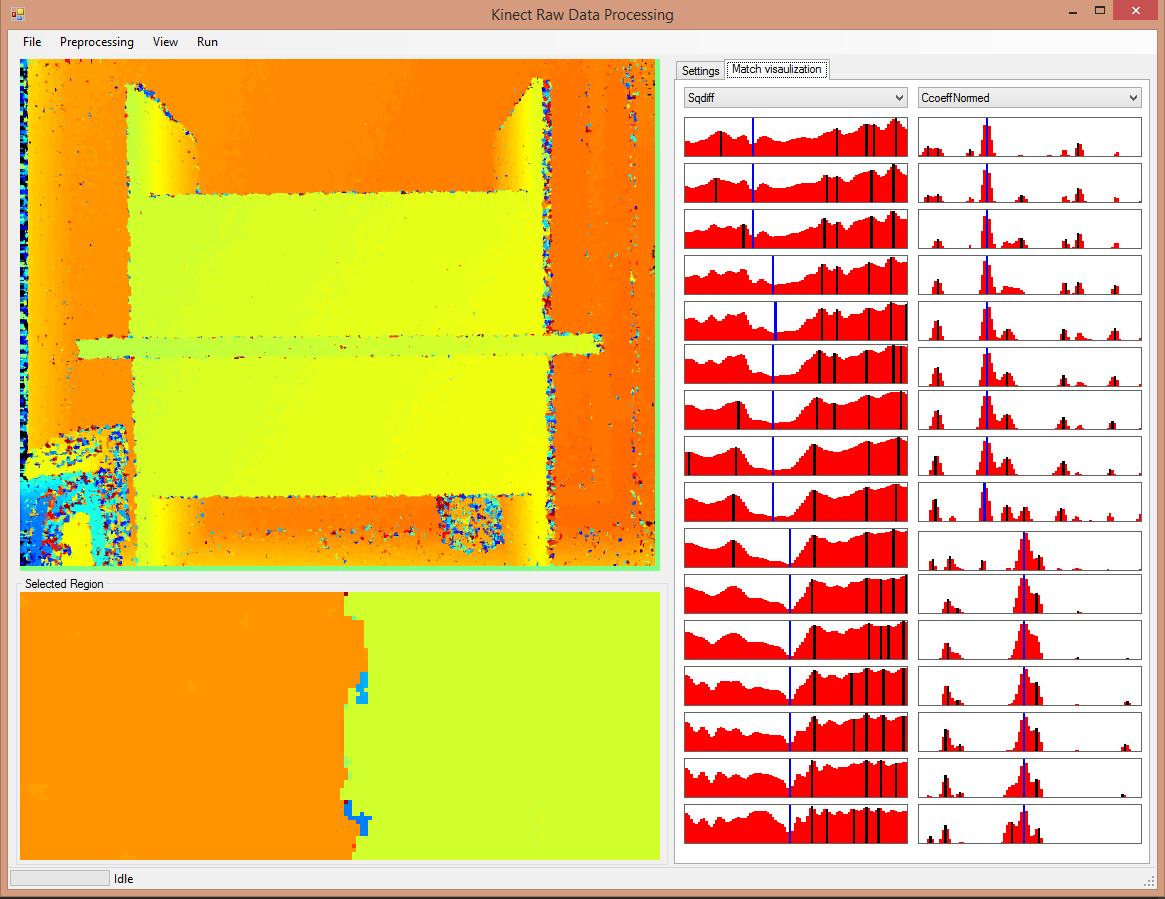
\includegraphics[width=0.9\linewidth]{figures/gui_data.png}
	\caption{Adatok megjelenítése}
	\label{fig:guiData}
\end{figure}

A bal alsó sarokban látható képrégió az aktuális puffer egy részének nagyított képét mutatja.
Ezt a funkciót az motiválta, hogy könnyebb legyen az illeszkedés vizsgálata az élek és pontszerű hibák körül.

Az előző féléves munka során, amikor a költségfüggvények hatékonyságát vizsgáltam, elengedhetetlen volt az illeszkedés minőségének valamilyen vizualizációja.
Erre szolgál a \figref{guiData} ábra jobb oldalán látható sáv.
Az aktuális megjelenített képen történő kattintással végrehajtódik a mintaillesztés a kattintott hely környezetében, és a jobb oldali sávon látható grafikonokra rajzolódik az illeszkedés jósága.
A két oszlopban két külön költségfüggvény választható az illesztéshez.
Az alsó, nagyított régió is a kattintás helyét veszi középpontjául.

%-----------------------------------------------------------------------------------------------
\subsection{Beállítások fül}\label{sect:settingsView}
%-----------------------------------------------------------------------------------------------

A beállítások fül alatt konfigurálható az egyes feldolgozási sorok tartalma.
Ahogy \figref{guiSettings} ábrán látható, a három sor külön állítható össze és hajtható végre.
Az implementáció jelenlegi formájában nem teljes, a fontosabb részekre fókuszáltam a félév során.

\begin{wrapfigure}{l}{0.45\textwidth}
	\centering
	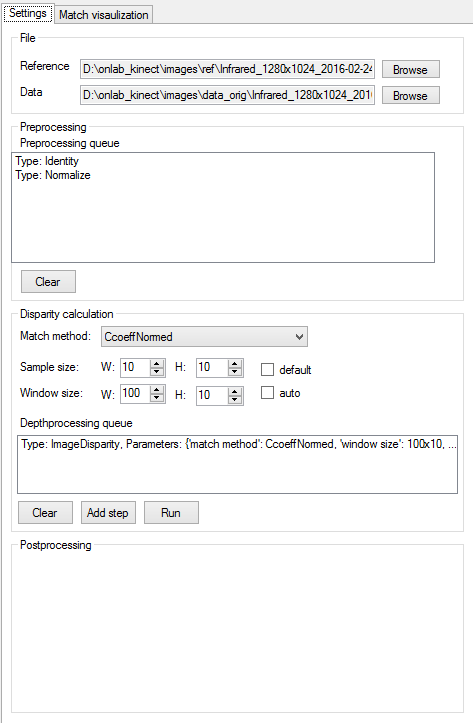
\includegraphics[width=0.45\textwidth]{figures/gui_settings.png}
	\caption{Adatok megjelenítése}
	\label{fig:guiSettings}
\end{wrapfigure}

Az felület jelentős átszervezésen megy keresztül az előző féléves verzióhoz képest.
Akkor a beállítások a felső menüsoron keresztül történtek.
Ennek nyomai még nem tűntek el teljesen.
Az előfeldolgozási lépések hozzáadása még mindig onnan érhető el.

A diszparitás számítás paraméterezése ezen fül alatt található.
Megadható az előző fejezetben tárgyalt ablak- és mintaméret, valamint választható az illeszkedés mérőszáma.
Jelen állapotában nagy hiányossága ennek a résznek, hogy nem választható meg a feldolgozási stratégia.
Elkezdődött ugyan az implementálása a lokális struktúrát figyelembe vevő stratégáknak, de ezek a felhasználói felületre még nem kerültek ki.

Az utófeldolgozási sor összeállítása sem került implementálásra a felületen.
Ennek oka, hogy voltak jóval érdekesebb és magasabb prioritást élvező feladatok.
Ebben a sorban jelenleg kizárólag a vizualizáció történik, ami jelen formájában amúgy sem lenne paraméterezhető.

Némi redundanciát adva a rendszerhez, a beállítások fül alatt is betölthető az adat- és referenciakép\footnote{Még a file menüből érhető el ez a funkció}.

%-----------------------------------------------------------------------------------------------
\subsection{Menüsor}\label{sect:menuStrip}
%-----------------------------------------------------------------------------------------------

A menüsör elemeit a \figref{menuStrip} ábra mutatja.
A file menü tagjait nem részletezem, céljuk egyértelmű.

\begin{figure}[ht!]
	\begin{subfigure}{.5\textwidth}
	  \centering
	  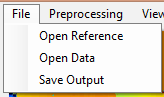
\includegraphics{figures/gui_file.png}
	  \caption{File menü}
	  \label{fig:fileMenu}
	\end{subfigure}
	\begin{subfigure}{.5\textwidth}
	  \centering
	  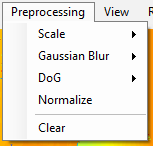
\includegraphics{figures/gui_preproc.png}
	  \caption{Előfeldolgozás menü}
	  \label{fig:preprocMenu}
	\end{subfigure}
	\begin{subfigure}{.5\textwidth}
		\centering
		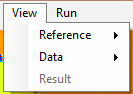
\includegraphics{figures/gui_view.png}
		\caption{Nézet menü}
		\label{fig:viewMenu}
	\end{subfigure}
	\begin{subfigure}{.5\textwidth}
		\centering
		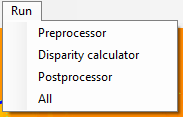
\includegraphics{figures/gui_run.png}
		\caption{Futtatás menü}
		\label{fig:runMenu}
	\end{subfigure}
	\caption{Menüsáv elemei}
	\label{fig:menuStrip}
\end{figure}

Az előfeldolgozás menü alatt az előző fejezetben tárgyalt lépések adhatók hozzá a feldolgozási sorokhoz.
Almenüikben a már tárgyalt paramétereik konfigurálhatóak.

A nézet menüben kiválasztható a megjeleníteni kívánt puffer.
Az almenük a feldolgozás szakaszait tartalmazzák: referencia- és adatkép esetén a nyers vagy előfeldolgozott, diszparitás esetén pedig a nyers vagy vizualizált állapot kérhető le.

A futtatás menüben indíthatók a feldolgozási sorok.
Lehetőség van egyesével indítani őket, vagy futtatható az összes is egyszerre.
Amennyiben egyesével indítjuk őket, a program nem engedi futtatni azokat a sorokat, amelyek bemeneti adata még nem áll rendelkezésre.
